% vim: set spell spelllang=en_gb tw=80:
\chapter{Implementation}\label{chap:impl}

% \guidance{%
%   This chapter should describe what was actually produced: the programs which
%   were written, the hardware which was built or the theory which was developed.
% 	Any design strategies that \textbf{looked ahead to the testing stage} might
% 	profitably be referred to (the professional approach again).\\
%   Descriptions of programs may include fragments of high-level code but large
%   chunks of code are usually best left to appendices or omitted altogether.
%   Analogous advice applies to circuit diagrams.\\ 
%   \textbf{Draw attention to the parts of the work which are not your own}. Making
%   effective use of powerful tools and pre-existing code is often laudable, and
%   will count to your credit if properly reported.\\
%   It should not be necessary to give a day-by-day account of the progress of the
%   work but \textbf{major milestones may sometimes be highlighted with advantage}.\\
% }

\prechapter{%
  In this chapter, I will describe how I implemented this project. What follows
  is an account of the programs I wrote, problems I encountered, solutions I
  implemented and tests I conducted.  Figure~\ref{fig:structure} shows an
  overview of this project's components and how they fit together.
}

\begin{figure}[t]
\centering
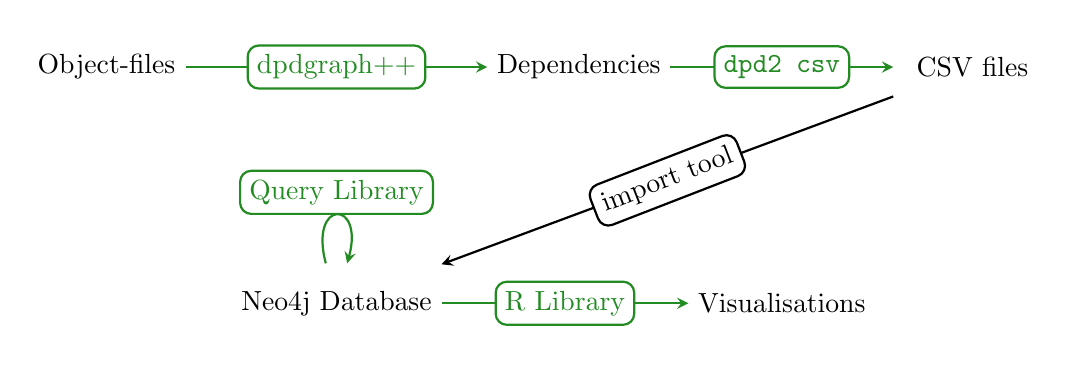
\begin{tikzpicture}[every loop/.style={}]
  \tikzstyle{phase} = [
    rectangle,
    % rounded corners,
    minimum width=2cm,
    minimum height=1cm,
    text centered,
    % draw=black,
  ]

  \tikzstyle{me} = [ thick, ->, >=stealth, color=ForestGreen ]
  \tikzstyle{metoo} = [ rounded corners, draw=ForestGreen, fill=white, text centered, text=ForestGreen ]
  \tikzstyle{notme} = [ thick, ->, >=stealth  ]

  \node (compiled-coq) [phase] {Object-files};
  \node (dpd-file) [phase, xshift=5cm, right of=compiled-coq] {Dependencies};
  \node (csv) [phase, xshift=4cm, right of=dpd-file] {CSV files};

  \draw [me] (compiled-coq) -- node[name=dpdgraph, metoo] {dpdgraph++} (dpd-file);
  \draw [me] (dpd-file) -- node[name=dpd2csv, metoo] {\texttt{dpd2 csv}} (csv);

  \node (neo4j-db) [phase, yshift=-2cm, below of=dpdgraph] {Neo4j Database};
  \node (visual) [phase, yshift=-2cm, below of=dpd2csv] {Visualisations};

  \draw [notme] (csv) -- node[rounded corners, draw=black, rotate=21.2, fill=white] {import tool} (neo4j-db);
  \path [me] (neo4j-db) edge[loop above] node[anchor=south, metoo] {Query Library} (neo4j-db);
  \draw [me] (neo4j-db) -- node[metoo] {R Library} (visual);

\end{tikzpicture}

\caption{Structure of Project. Nodes show the format of the information. Edges
  show the transformations. Edges in green  show my contributions.}\label{fig:structure}
\end{figure}

\section{Coq object-files to CSV}

This section of implementation corresponds to `dpdgraph++' and `\texttt{dpd2
csv}' on Figure~\ref{fig:structure}: modelling the data contained in and the
structure of a Coq library as CSVs.  First, I will briefly describe the
algorithm I used to construct a dependency graph constructed from a compiled Coq
library. Then, I will elaborate upon how I modelled the Coq library by going
through the attributes of each node and edge in the dependency graph. Finally, I
will describe the format of the \texttt{.dpd} file output, which contains the
graph constructed from the compiled Coq library.

\subsection{Algorithm}

This is a high-level overview of the algorithm I used in `dpdgraph++' to
construct a dependency graph from a compiled Coq library.

\textbf{Input:} A Coq script containing a list of files in the library (I wrote
a shell-script to generate this file automatically) and the path to the compiled
Coq library.

\textbf{Output:} A \texttt{.dpd} file containing a description of a graph whose
nodes represent Coq proof-objects and whose edges represent various
relations between the proof-objects.

\begin{enumerate}

  \item For each module, for each proof-object in the module:

    \begin{enumerate}
      \item if the proof-object is not in the set of nodes, add it.
      \item for each module in the chain of modules from the proof-object's parent
        to the root of the library: 
        \begin{enumerate}
          \item if the module is not in the set of nodes, add it.
          \item if there is not an edge between a module and its child in the
            set of edges, add it.
        \end{enumerate}
      \item collect the proof-object's dependencies by recursing over its AST.
      \item for each dependency: 
        \begin{enumerate} 
          \item if the dependency is not in the set of nodes, add it.
          \item if there is not an edge between the proof-object and its
            dependency in the set of edges, add it.
          \item otherwise, retrieve the edge and increment its \emph{weight
            attribute} (representing the number of uses)
        \end{enumerate}
    \end{enumerate}
  
  \item For each node in the set of nodes, output all its attributes
    (attributes described in Subsection~\ref{subsec:modelling}; output format described in
    Subsection~\ref{subsec:translation}).

  \item For each edge in the set of edges, output all its attributes (source,
    destination and weight; output format described in
    Subsection~\ref{subsec:translation}).

\end{enumerate}

\subsection{Modelling}\label{subsec:modelling}

Although I used dpdgraph as a starting point, I rewrote all the
attribute-assigning code because the meaning of the attributes it initially
collected was not obvious and the terminology it used did not correspond to
recognisable Coq constructs.

I added the following attributes and improved the dependency-collection for
inductive types and their constructors (as I will describe
in~\ref{subsubsec:typecon}~\nameref{subsubsec:typecon} on
page~\pageref{subsubsec:typecon}).

\subsubsection{Precise Kinds}\label{subsubsec:kinds}

A proof-object can be one of the following things, corresponding to an AST term:
\textsf{module}, \textsf{class}, \textsf{type\_constructor},
\textsf{inductive\_type}, \textsf{definition}, \textsf{assumption} or
\textsf{proof}.

Optionally, some terms have more precise terminology, for distinguishing
different constructs. For example, when writing Coq, there is no \texttt{Proof}
keyword; instead \texttt{Theorem}, \texttt{Lemma}, \texttt{Fact},
\texttt{Remark}, \texttt{Property}, \texttt{Proposition} and \texttt{Corollary}
all are \emph{synonyms} for proofs. Full details can be found in
Appendix~\ref{chapter:fullmodel}.

So, to model this categorisation, I assigned each node a `kind' \emph{label}:
labels are strings used to group nodes into subsets; since a node can belong to
more than one subset, it can have more than one label assigned to it. To model
the more precise distinctions, I optionally assigned some nodes a `subkind'
label.

\subsubsection{Recursive Modules}\label{subsubsec:recmodules}

Every proof-object is contained within a module and every module is either
contained in a file, is a file or is a directory. To model this inclusion
relation, analyse module-level dependencies (like coqdep) and compare the
results of community detection algorithms with the module structure of a
library, I augmented `dpdgraph++' to include modules in the graph. Using the
Coq API, I could get the fully-qualified path (path from the library's root) of
a proof-object. Using a variant datatype, I expanded the type of a node in the
graph to include modules and propagated the changes throughout the project.

However, because the Coq API returned module paths as strings, modules were in
the model as a flat structure: modules could be related to objects but not to
other modules. I fixed this by inferring (splitting the fully-qualified path)
and adding all the ``ancestors'' of a module with the correct relations
(parent as source, child as destination, repeatedly up to the root module).

\subsubsection{Types and Constructors}\label{subsubsec:typecon}

One of the most glaring omissions from dpdgraph's initial model was the
inability to relate a type to its constructor(s). To fix this,
I improved the dependency-collection code (see Appendix~\ref{chapter:sample}).

Expanding an AST term for type-constructors shows which type it constructed
(note that types have no information about which constructors construct them).
Since dependencies were constructed in a depth-first manner \emph{down} the AST,
I had to store the type and type-constructor relation reversed but output it
in the correct order.

To do so, I compared each pair of nodes to see if it (a) was a type and a
constructor and if so, (b) the constructor's fully-qualified type matched the
fully-qualified name of the type. If both these criteria were met, I swapped the
direction of the edge output.

\subsubsection{Types}

% Conducting a \emph{cognitive walkthrough} (detailed in
% Chapter~\ref{chapter:evaluation}) spurred the addition of \emph{type
% signatures} to the model.

Another unmissable omission from dpdgraph's initial model was the inability to
see the type of a proof-object. Type theory is central to a Coq user's work and
being able to include them in the model, would, along with kinds, subkinds and
modules, help towards meeting the modelling requirement~\ref{req:m1} of
including as much relevant data as possible. 

Coq's type-checking algorithm is complex. To replicate it within
`dpdgraph++', I followed the functions called for the Coq command
\texttt{Check} \emph{<expression>} (for printing the type of a given
expression).  This led to the algorithm for \emph{getting} the type, which I
then implemented.

A subtlety I had to overcome was \emph{using} the output in \texttt{.dpd} and
CSV files. I replaced newlines, quotation marks, and commas with hash signs,
single-quote marks and underscores respectively, because the former were used to
delimit data in \texttt{.dpd} and CSV files and would have otherwise caused
errors when they were being parsed into subsequent programs.

\subsubsection{Relations}

Modelling relations was the most interesting aspect of deciding how to
represent information. I wanted to keep consistent the notion of expanding a
node to see more details: if a user is looking at an object, they should be able
to expand the object to see what the object depends on; if a user is looking at
a module, they should be able to expand the module to see the objects contained
within that module; if a user is looking at a type, they should
be able to expand the type and see its constructors.

I modelled this idea with the following relations:
\mintinline{cypher}{(src)-[:USES]->(dst)} for dependencies,
\mintinline{cypher}{(type)-[:CONSTRUCTED_BY]->(constr)} for types, and
\mintinline{cypher}{(module)-[:CONTAINS]->(object)} for modules.

I had two problems whilst implementing these relations. First was finding
and matching types and constructors (details of which are described
in~\ref{subsubsec:typecon}~\nameref{subsubsec:typecon} on
page~\pageref{subsubsec:typecon}).

Second was balancing expressiveness against simplicity. I considered
relations of the following format, \texttt{X\_USES\_Y} for kinds X and Y.
Although this was useful for fewer kinds, I decided its specificity when
subkinds are included in the model made the model too large and complex (on the
order of $n^{2}$ relations). Since Cypher allows pattern-matching and
filtering based on kinds and subkinds anyway, I chose the simplified model
presented above.

\subsection{Translation}\label{subsec:translation}

This subsection corresponds to `\texttt{dpd2 csv}' on
Figure~\ref{fig:structure}.  Once a model is constructed (in the form of a
graph) by `dpdgraph++' and output to a \texttt{.dpd} file, it is translated by
the \texttt{dpd2} tool to a CSV file for use by Neo4j's import tool to create a
database. I will now present an overview of the \texttt{.dpd} and CSV formats,
as well as the \texttt{dpd2} tool itself.

\subsubsection{\texttt{dpd} Format}

`dpdgraph++' outputs the graph representing the model as a \texttt{.dpd} file
with the following format for nodes (one per line):

{\tt N: \emph{<id>} "\emph{<name>}" [\emph{<property>}=\emph{<value>}];}

for example (full type elided for brevity), 

{\tt N: 76 "matches" [type="... -> bool", subkind=fixpoint, kind=definition, path="RegExp.Definitions", ];}

and likewise for edges:

{\tt E: \emph{<src id>} \emph{<dst id>} [\emph{<property>}=\emph{<value>}];}

for example, 

{\tt E: 150 145 [type=CONTAINS, weight=1, ];}.

\subsubsection{CSV}\label{subsubsec:translationcsv}

Once it is output as a \texttt{.dpd} file, a model can be translated to various
other formats. For example, dpdgraph includes a tool to output a \texttt{.dot}
file (a format used extensively for \emph{visualising} graphs by many tools)
from a \texttt{.dpd} file. This is what I used to generate
Figure~\ref{fig:static}.

However, for the purpose of this project, I translated the \texttt{.dpd} file
(using the \texttt{dpd2} tool described below) to \emph{two} CSV files: one for
nodes and one for edges, for use with Neo4j's import tools with the following
headers.

\texttt{objectId:ID(Object), name, kind:LABEL, subkind:LABEL, path, type}

Here we see name, path and type declared as properties, kind and subkind
declared as labels and the objectId field declared as a unique identifier (or in
relational terms, a key) for the nodes (in this schema, called `Objects') in
the graph.

\texttt{:START\_ID(Object), :END\_ID(Object), weight:int, :TYPE}

Similarly, here we see relations (between `Objects' as declared
previously) named according to the value under the \texttt{:TYPE} column (for example,
\texttt{CONTAINS}, \texttt{USES} or \texttt{CONSTRUCTED\_BY}), each with an
integer property, weight.

Using a CSV format makes adding extra properties, labels and relations very
straightforward. This means it is easy to integrate other tools with this
project and so extend this project with new features.

\subsubsection{\texttt{dpd2} Tool}\label{subsubsec:dpd2}

Initially, this tool started out as the \texttt{dpd2dot} utility (bundled with
dpdgraph). I refactored it into a more general, \texttt{dpd2} tool which could
accept the file-type (\texttt{.dot} or CSV) as a command-line argument.

Whilst using this tool, I discovered it had a bug. By default, \texttt{dpd2}
attempts to remove reflexive and transitive dependencies (i.e. $a \rightarrow a$
and removing $a \rightarrow c$ if $a \rightarrow b$ and $b \rightarrow^{+} c$)
in a depth-first manner.  For large graphs, doing so is stack-intensive, and
thus causes a stack-overflow error.  Since this ``feature'' was unnecessary
(because it \emph{removed} useful information) and appeared time-consuming to
fix, I passed the \texttt{-keep-trans} flag on subsequent uses to avoid the issue
altogether.

\section{CSV to Neo4j}

The `import tool' in Figure~\ref{fig:structure} is a command-line program that
is included with Neo4j. Given a target directory, a CSV file containing the
nodes of the graph and a separate CSV file containing the edges of the graph,
the import tool constructs a database. As explained
in~\ref{subsubsec:translationcsv}~\nameref{subsubsec:translationcsv}, the
headers determine the labels, properties and IDs of nodes as well as the
sources, destinations, properties and types of edges.

\section{Query Library}

This section of the implementation corresponds to the `Query Library' and the
`R Library' shown in Figure~\ref{fig:structure}. I will now outline the
plugins I worked with to meet the interaction and computation requirements
(page~\pageref{req:i1}).

\subsection{Java Library}

APOC (Awesome Procedures on Cypher) provides many convenient procedures. Of
note are:

\begin{itemize}

  \item functions for constructing and examining a \emph{meta-graph} showing
    which labels and relations are in the database and how they are connected.
    They allow a user to see an overview of the model.

  \item a few key graph algorithms, such as: node and path expansion, spanning
    tree, Dijkstra's shortest paths, A* search, label propagation (for community
    detection) and centrality measures (betweenness, closeness and PageRank).

  \item functions for regular-expressions and mathematics, useful for selecting
    nodes based on statistics (for example, PageRank) or selecting nodes based on their
    path property.

\end{itemize}

Each of these can be called directly from within Cypher; for example, writing
\texttt{CALL apoc.meta.graph()} would return the meta-graph of the database.

\subsection{R Library}

For the `R Library', (to meet requirement~\ref{req:c1} for a core set of good
defaults) I wrote several example programs which automatically processed data
from a new database, stored the information again for later use (to avoid
re-computation) and output appropriate visualisations.  Since processing could
take on the order of minutes, I also provided status updates (informing the user
of the tasks being executed), execution times for each task, as well as
progress-bars where possible and relevant (for example,\ committing a
transaction to the database). See Appendix~\ref{chapter:sample} for details.

\subsubsection{Visualisation}

There are many interesting ways to visualise the plethora of data that
translating Coq libraries (representing mathematical theories) into graph
databases produces.

Surprisingly, igraph was able to help with visualising graphs as well analysing
them.  Whilst visNetwork -- with its own JavaScript, force-directed, physics
rendering -- produced more aesthetically pleasing results for smaller graphs,
the webpages it output for larger graphs took intolerably long to render inside
a typical web-browser (Firefox/Opera). Thanks to an (experimental) integration
with igraph (specifically, igraph's layout mechanisms), I could pre-compute
graph layouts in fast, native C/C++ \emph{before} rendering graphs in a
web-browser.

\section{Project Related}

During implementation, I learnt several skills and lessons about correct project
management. Small things, such as grep-ing a code base or keeping track of time
and a log of work done, proved to be useful. However, to ensure this project ran
smoothly on a larger-scale, I focused more on the following areas.

\subsection{Testing}

For most of this project, I conducted testing manually by inspecting the output.
Though this was tedious, it was the only way to do so when the model was
undergoing continual development. Once I fixed the model, I shifted my focus to
visualisation and used automated tests. These tests were particularly useful
when I had to duplicate this project because for compatibility with libraries I
was using to test this project (see Subsection~\ref{subsec:cibuilds}).

I used some of my older Coq proof-scripts -- problems I solved when learning Coq
-- to check output on a small scale (where I knew every single aspect of the
library, and testing turnaround was quick). I used Coq's Standard Library as a
large-scale stress-test, to ensure all constructs were translated correctly.
When I did find problems, I could usually trace them back using output from debug
statements I had embedded into `dpdgraph++'.

\subsection{Continuous-Integration Builds}\label{subsec:cibuilds}

Although this project never failed to build locally, there were occasionally
problems when trying to build it on the project supervisor's machine. The
problem was compounded when it became apparent that smaller libraries (such as
CoqRegExp and the solved problems) relied on a version of Coq (8.5.2) older than
the one Mathematical Components (needed for this project's moon-shot, the Odd
Order Theorem) relied on (8.6). I set up Travis-CI for continuous-integration
builds, made version dependencies precise and explicit, and removed much of the
inconvenience and uncertainty surrounding builds on other machines.

\subsection{Tooling}

At first, I ran the project half on Windows and half on a Linux VM (virtual
machine), using shared folders. I had a few reasons for this: I had already set
up Coq and Neo4j on Windows, both are easier to interact with in a graphical
environment and starting up a VM just for some experimentation took too long.

Eventually, this set-up became confusing and time-consuming and I made the leap
to running the project fully on a Linux VM. Nevertheless, I had serious issues
when working on R integrations: running a Java database inside a Linux VM was
insufferably slow and switching databases was not easy. I solved this problem by
setting up SSH reverse-port-forwarding (to let R inside the Linux VM connect to
a Neo4j instance running directly on Windows) for decent performance.

To be the most productive during longer sessions of work, I also set up editor
integrations for OCaml, dramatically reducing the edit-compile cycle (especially
for a strong, statically-typed programming language as OCaml). At this point,
Coq's use of non-standard OCaml features, extensions and build-systems became
particularly frustrating. For example, I spent a considerable time was spent
untangling the Makefile inherited from dpdgraph to have cleaner, out-of-source
builds and reduce the mess in the current working directory, all to no avail as
I realised how complex of the build-system for Coq plugins is.

\section{Dead-ends}

I have now finished describing the whole project; all parts of
Figure~\ref{fig:structure}. I will now explain why I did not further pursue a
couple of seemingly obvious, alternative strategies to modelling Coq libraries.
Both centre around the same theme: analysing the Coq source-files directly
instead of compiling them and then analysing the object-files.


\subsection{Coqdoc}

I tried to modify coqdoc's output into a useful format but this did not prove
fruitful because the purely lexical tokenisation coqdoc does cannot infer or
preserve as much information as full parsing.

\subsection{Coq source-files to CSV}

So, why not try parsing the source-files directly? This is an appealing idea,
because with my current approach, there is still some information being lost
during compilation: there is an \emph{apparent} absence or duplication of some
modules and a lack of notation and tactics.

The former arises from the use of \emph{functors}: modules that take other
modules as arguments (used to abstract over arguments, tactics, definitions and
proofs). A concrete example (from the Coq Standard Library) is the theory of
total orders, minimums and maximums, which is applied to naturals, integers and
rational numbers (as well as any other ordered types). Such functors cannot be
compiled unless fully applied (explaining the \emph{absence} of some modules);
when fully applied, they essentially copy their \emph{structure} into each
instance (explaining the \emph{duplication} of some module names and
structures).

\subsubsection{Exploring Solutions}

\emph{Several} issues stop parsing from being a pragmatic solution, least of
which are the size of the AST and complexity of parsing Coq files (Coq uses
non-standard OCaml tools to implement an \emph{extensible grammar}, making the
whole situation quite ugly to work with).

\begin{enumerate}

  \item \emph{Modules and functors are represented identically} in the AST, with
    the former as a special case of the latter, making it very difficult to
    distinguish between the two on an AST-level. By far, this was the biggest
    roadblock.

  \item \emph{Module types}, or \emph{signatures}, must be incorporated into
    the model for functors to make sense. Modules and signatures share a
    many-to-many relation: a signature can be satisfied by multiple modules
    and a module can satisfy multiple signatures. To express this correctly
    would require \emph{signature-matching}, a notoriously difficult task (and
    the reason why few languages support ML-style modules).

  \item Further issues involve resolving objects into a global namespace and
    knowing which compiler flags were given during compilation (to match
    physical directories to logical modules), all of which complicate matching
    and merging with the compiled proof-objects.

\end{enumerate}

\subsubsection{Resolution}

I made some progress in tackling these issues, but it took too long, so I could
not justify spending more time on it. Functors are not used in many projects,
(especially given the popularity and ease of use of \emph{type-classes} for
expressing generalisations). 

Furthermore, including functors risked violating requirement~\ref{req:m1} (by
retaining information that could be difficult to understand or use).
Additionally, given that names \emph{and structures} of instantiated modules are
duplicated, it could be possible to \emph{reconstruct} generalisations
\emph{representing functors} once the database is created (hence respecting
requirement~\ref{req:m3} by not pre-computing too much data).

As such, extracting information directly from Coq source-files did not
contribute to the overall project, but presents clear ways forward for future
work.

\section{Summary}

I just presented an in-depth account of the programs I wrote (dpdgraph++, dpd2,
Query \& R libraries), problems I encountered (recursive modules, relating types
and constructors, incorporating type-signatures, CSV translation, dependency and
version tracking, impenetrable build-systems and parsing information directly
from Coq source-files), solutions I implemented and tests I conducted.
Throughout, I referenced the project requirements to justify important
decisions.
